\section{The Standard Model- A Brief Overview}
The Standard Model of particle physics which has been one of the most successful and well-tested theories so far, provides the most fundamental description of nature by incorporating the elementary particles and their interactions. These elementary particles are categorized into two families: fermions (having half integer spins) which form matter as we know it, and bosons (with integer spins) serving as mediators of the three fundamental forces. While electromagnetic interactions are mediated by the photon ($\gamma$); strong and weak interactions are mediated by gluons (g) and by $W^{\pm}, Z^{0}$ bosons respectively. A fundamental particle that mediates gravitation has been only postulated theoretically, and is left out of the Standard Model, since the effects of gravity are too weak to play any important role in the realm of particle physics. 

\begin{figure}[h!]
\centering
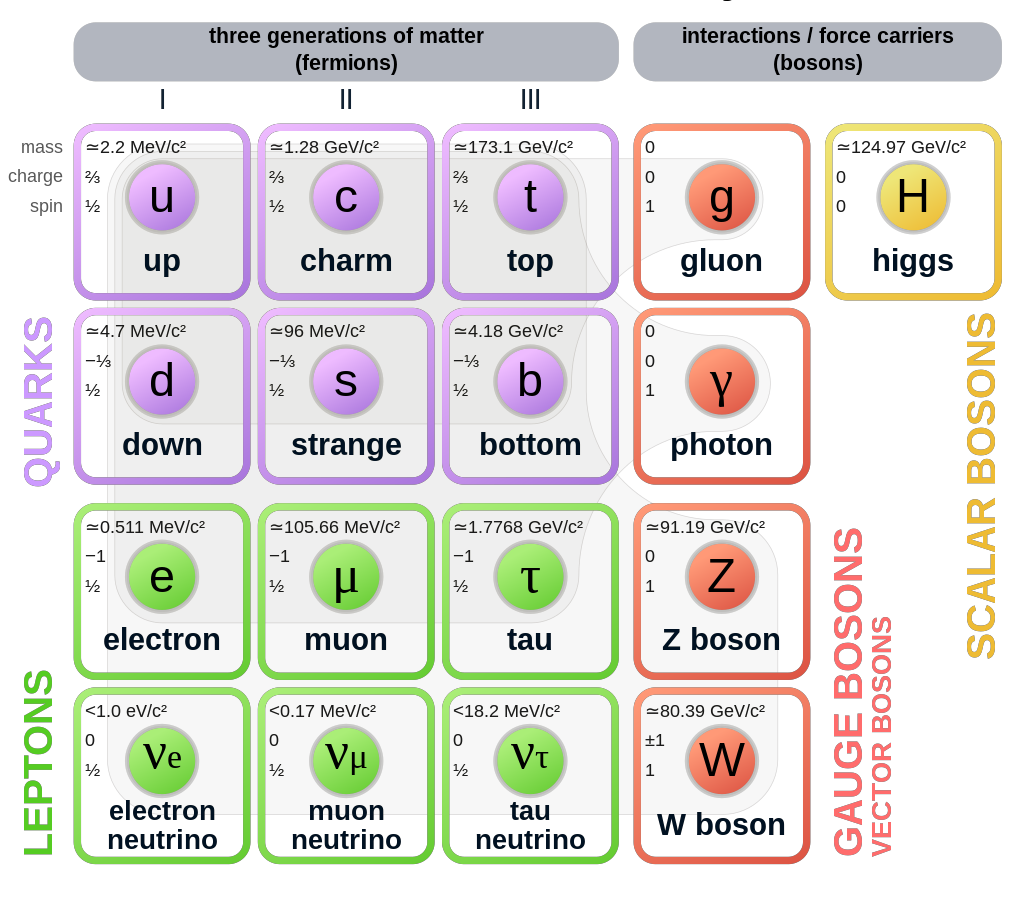
\includegraphics[scale=0.4]{./images/Standard_Model_of_Elementary_Particles.png}
\caption{A chart showing the families of elementary particles in the Standard Model}
\label{fig:StdModel}
\end{figure}

The fermions consists of three generations of quarks and leptons. The quarks have six flavours: up (u), down (d), charm (c), strange (s), top (t) and bottom (b). Similarly, the leptons consist of the electron ($e$), muon ($\mu$) and tau ($\tau$), each having its own associated charge-less and almost massless neutrino ($\nu_{e}$, $\nu_{\mu}$ and $\nu_{\tau}$). Furthermore, each particle in the standard model has its own antiparticle. The quarks are able to form composite particles in either three quark combinations, called baryons ($qqq$/$\bar{q}\bar{q}\bar{q}$) or a quark-antiquark pair, called a meson ($q\bar{q}$). Mathematically, the elementary particles are described as elements of representations of certain symmetry groups. The gauge fields that couple to these particles (i.e. mediate the interactions) arise naturally as a consequence of invariance of their corresponding Lagrangian under local group transformations \cite{thomson_2013}. As such, the gauge symmetry that governs the Standard Model is given by: $$SU(3)_{\mathrm{Colour}}\times SU(2)_{\mathrm{Left\ chiral}}\times U(1)_{\mathrm{Y}(\mathrm{Weak \ hypercharge})}$$

\section{The Unified Theory of Electromagnetic and Weak Interactions}
Since the experiment deals with verifying some of the properties of the $Z^{0}$ bosons, it is of interest to touch upon the theory of electroweak unification.

While electromagnetism and the theory of weak interactions were formulated separately, it was later on postulated that at higher energies ($\sim$ 246 GeV \cite{pdg-ew}), both these interactions would be unified into a single force. As such, the GSW(Glashow-Salam-Weinberg) electroweak model was developed in the 1960s to describe this unified force. 

One finds that imposing the principle of local gauge invariance on the $SU(2)_{L}$ symmetry group leads to the introduction of three gauge fields: $W^{(1)},\ W^{(2)}$ and $W^{(3)}$ (or $W^{0}$ in some references) \cite{thomson_2013}. The physical $W^{+}$ and $W^{-}$ bosons (that mediate the weak charged current interaction) can be seen as the linear combinations: 
\begin{equation}
W^{\pm}=\dfrac{1}{\sqrt{2}}\left(W^{(1)}\mp W^{(2)}\right)
\end{equation}
However, the $W^{(3)}$ field has no physical interpretation of its own. Therefore an additional symmetry, the $U(1)_{Y}$ group is introduced. The field $B$ (or equivalently $Y^{0}$) arising as a consequence of this new symmetry, similarly does not have a physical meaning on its own. Rather, it was seen that linear combinations of the $W^{(3)}$ ($W^{0}$) and $B$ ($Y^{0}$) fields gives rise to the  photon and the $Z^{0}$ boson:

\begin{equation}
\begin{pmatrix} 
\gamma \\ 
Z^{0} 
\end{pmatrix}
= 
\begin{pmatrix}
\cos \theta_{W} & \sin \theta_{W} \\
-\sin \theta_{W} & \cos \theta_{W} 
\end{pmatrix}
\begin{pmatrix}
B \\
W^{(3)}
\end{pmatrix}
\end{equation}
where $\theta_{W}$ is the weak mixing/Weinberg angle

In addition to this, it is to be noted that the gauge fields $W^{(1),(2),(3)}$ and $B$ have to be massless, in order to respect gauge invariance under local $SU(2)_{L}\times U(1)_{Y}$ gauge transformation. However, the physical gauge bosons $W^{\pm}$ and $Z^{0}$ are predicted to be massive, whereas the photon should remain massless. To explain this, the concept of electroweak spontaneous symmetry breaking was introduced. A massive scalar field (the Higgs field) is introduced, to which these bosons ($W^{\pm}$, $Z^{0}$) must couple to, in order to get their physical masses, while the photon does not interact with it \cite{Dooling:207610}. The intricacies of the Higgs mechanism are not of immediate interest here, and can be understood from standard references \cite{thomson_2013, Griffiths:111880}.

\section{Physics Related to the $Z^{0}$ Resonance}
\subsection{$e^{+}e^{-}$ Interactions}
Before discussing the processes of interest involving $Z^{0}$ production, we first list out the important ways in which $e^{+}e^{-}$ pairs can interact \cite{UB}:
\begin{itemize}
\item $\bm{e^{+}e^{-}\rightarrow e^{+}e^{-}}$: Bhaba scattering (elastic scattering) of $e^{+}e^{-}$ pairs 
\item $\bm{e^{+}e^{-}\rightarrow e^{+}e^{-}\gamma \gamma}$: two photon process; $e^{+}e^{-}$ can scatter off of virtual photons, arising out of the incoming $e^{-}$ and $e^{+}$ themselves and these photons can then produce hadrons
\item $\bm{e^{+}e^{-}\rightarrow f \bar{f}}$: Electron-positron pairs annihilate to produce a gauge boson ($\gamma$ or $Z^{0}$), which would in turn produce a fermion-antifermion ($f\bar{f}$) pair. Here $f\bar{f}$ are fermions other than $e^{+}e^{-}$ since that process is already included under Bhaba scattering.
\item $\bm{e^{+}e^{-}\rightarrow \gamma \gamma / \gamma \gamma \gamma}$: An electron-positron pair could also produce two or three photons 

These $e^{+}e^{-}$ interactions are displayed in Figure \ref{fig:eeint}.

\end{itemize}

\begin{figure}[H]
\centering
\begin{subfigure}{0.4\textwidth}
    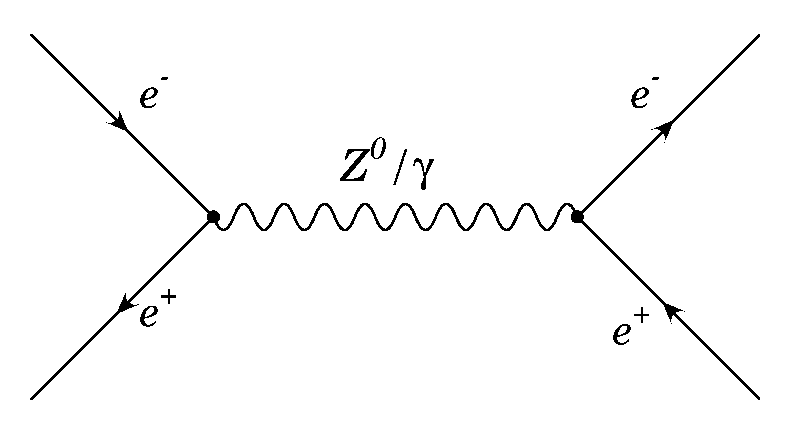
\includegraphics[width=\textwidth]{bhabha-s}
    \caption{$s$-channel Bhaba scattering}
\end{subfigure}
%\hfill
\begin{subfigure}{0.4\textwidth}
    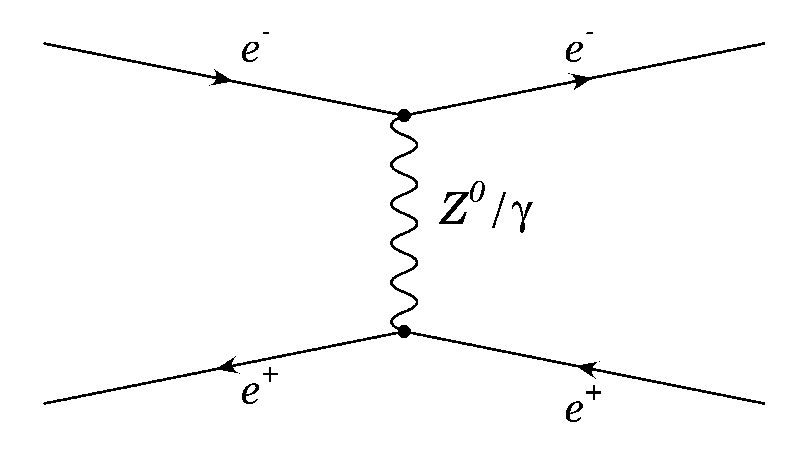
\includegraphics[width=\textwidth]{bhabha-t}
    \caption{$t$-channel Bhaba scattering}
\end{subfigure}
%\hfill
\begin{subfigure}{0.4\textwidth}
\centering
    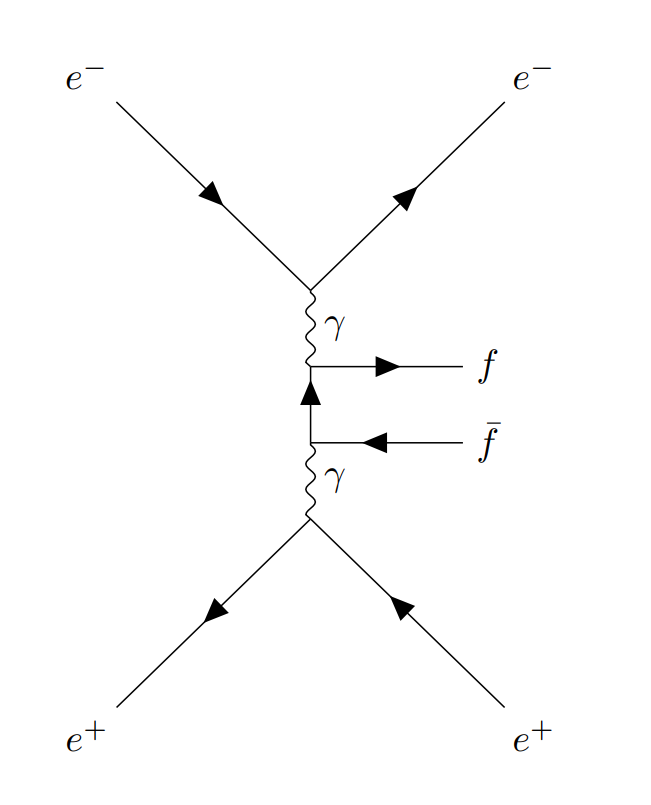
\includegraphics[width=0.9\textwidth]{twophoton}
    \caption{Two photon process}
\end{subfigure}
%\hfill
%\vspace{5em}
\begin{subfigure}{0.4\textwidth}
\centering
    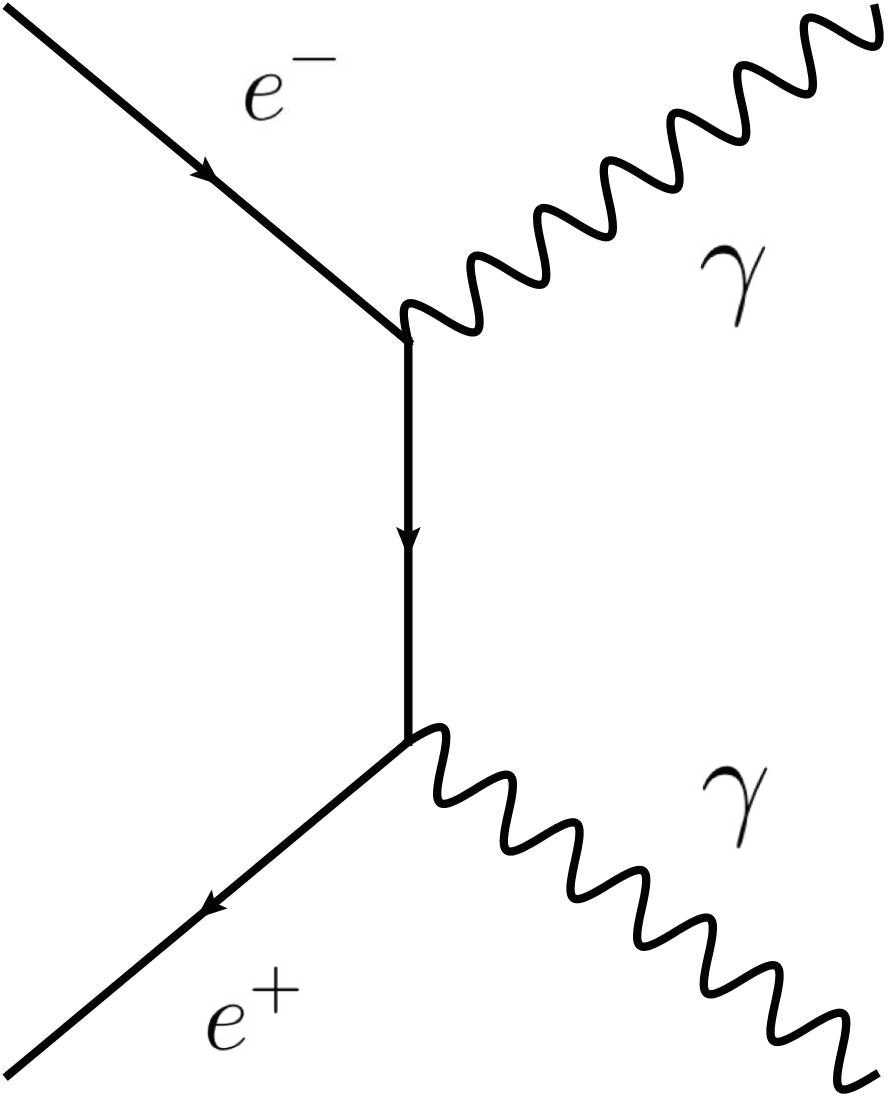
\includegraphics[width=0.7\textwidth]{eeyy}
    \vspace{2em}
    \caption{Production of two photons from $e^{+}e^{-}$ pair}
\end{subfigure}
%\hfill 
\begin{subfigure}{0.45\textwidth}
    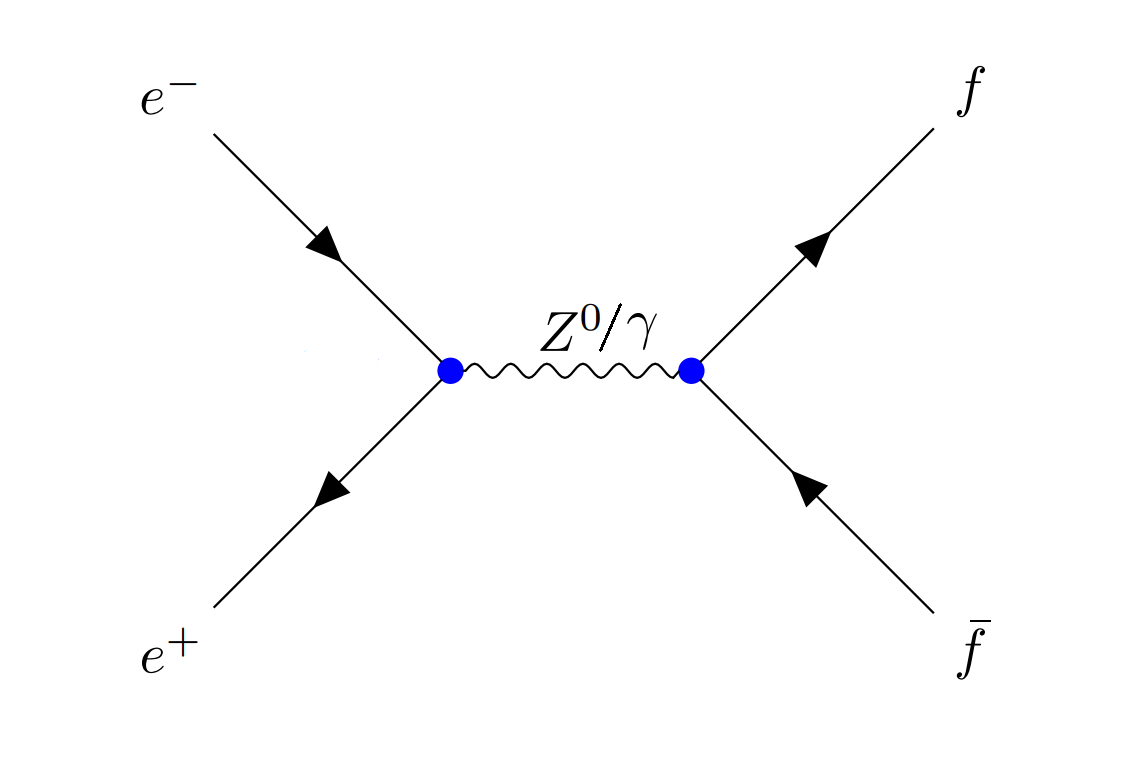
\includegraphics[width=\textwidth]{anihillation}
    \caption{Electron-positron annihilation to $f\bar{f}$}
\end{subfigure}
%\hfill      
\caption{Some examples of $e^{+}e^{-}$ interactions \cite{UB,Janot:2705419,qmdiaries}}
\label{fig:eeint}
\end{figure}

In case of the lowest order $e^{+}e^{-}\rightarrow f \bar{f}$ process, there are contributions to cross section from pure $Z^{0}$, pure $\gamma$ as well as from $\gamma - Z^{0}$ interference terms. However, near center of mass energies close to the $Z^{0}$ resonance, the major contribution to the total cross section is from the pure $Z^{0}$ term.

Additionally, it is easy to see that for the particular case of $e^{+}e^{-}\rightarrow e^{+}e^{-}$ scattering (Bhaba scattering), there is a t-channel contribution in addition to the s-channel component. The cross sections of both these processes have have different angular dependencies \cite{UB}
\begin{align}
\left(\dfrac{d\sigma}{d\Omega}\right)_{s}&\propto (1+\cos^{2}\theta)\\
\left(\dfrac{d\sigma}{d\Omega}\right)_{t}&\propto (1-\cos\theta)^{-2}
\end{align}
This means that while the $s$ channel cross section has a major contribution at large angles (or small values of $\cos\theta$), the $t$-channel contribution increases asymptotically at small angles (or large values of $\cos\theta$). As shall be seen later on, removing the t-channel contribution is an essential step, since we are only concerned with finding the inherent forward-backward asymmetry associated with the $s$-channel processes.

\subsection{Forward-Backward Asymmetry}
When we consider the $s$-channel processes $e^{+}e^{-}\rightarrow f\bar{f}$, as discussed before, if the process is mediated purely by photons ($\gamma$) then the differential cross section follows the $(1+\cos^{2}\theta)$ dependence and it shows a symmetric dependence on the scattering angle $\theta$. However, for the same process mediated by $Z^{0}$ bosons we find that there is an additional term contributing to the asymmetry:
\begin{equation}
\left(\dfrac{d\sigma}{d\Omega}\right)_{s\ (Z^{0})}\propto a(1+\cos^{2}\theta) + 2b\cos\theta
\end{equation}

From theory of electroweak interactions, this asymmetry (between the number of fermions produced in the forward direction, $\theta>\pi /2$ and the backward direction, $\theta<\pi /2$) can be understood to be arising from the fact that the $Z^{0}$ does not couple equally to right handed and left handed fermions. This becomes more clear by looking at the form of the asymmetry term:
\begin{equation}
b=\left[\left(g_{L}^{e}\right)^{2}-\left(g_{R}^{e}\right)^{2}\right]\left[\left(g_{L}^{f}\right)^{2}-\left(g_{R}^{f}\right)^{2}\right]
\end{equation}
where $g_{L}^{f}$ and $g_{R}^{f}$ signify the coupling of $Z^{0}$ to left handed and right handed fermions respectively. It can be clearly seen that in case the these two couplings had been equal, the asymmetry term would have gone to zero \cite{thomson_2013}.

The forward backward asymmetry factor is given as the ratio:
\begin{equation}
\mathcal{A}_{fb}=\dfrac{\sigma_{F}-\sigma_{B}}{\sigma_{F}-\sigma_{B}}=\dfrac{3b}{4a}
\end{equation}
where $\sigma_{F}$ and $\sigma_{B}$ are the cross sections in forward and backward directions respectively.

It is found that at the resonance of $Z^{0}$ boson, $\mathcal{A}_{fb}$ simplifies to \cite{UB}:
\begin{equation}
\mathcal{A}_{fb}^{f}\approx 3\left(\dfrac{g_{V}^{f}}{g_{A}^{f}}\right)=1-4\sin^{2}\theta_{W} 
\end{equation}
Thus from the calculation of the forward-backward asymmetry, the ratio of $g_{V}^{f}$ (vector coupling strength between $Z^{0}$ and fermions) to $g_{A}^{f}$ (axial vector coupling strength between $Z^{0}$ and fermions) can be found, which in turn gives us the Weinberg (weak mixing) angle $\theta_{W}$.
\subsection{Background Processes: Radiative Corrections}
In order to test out the predictions of the Standard Model at a very high level of precision, higher order background processes need to be accounted for and as such the corrections made due to these processes are called 'radiative corrections'. The following are some of these processes that need to be accounted for \cite{Zedometry}:
\begin{itemize}
\item \textbf{Initial state radiation (ISR):} The radiation of photons in the initial state lead to decrease in the centre of mass energy and thus affect the $Z^{0}$ resonance peak parameters. This leads to a peak height reduction by upto 25 \%, shift of peak to higher energy and increase in full width at half maximum (FWHM). 
\item \textbf{Final state radiation (FSR):} When photons or gluons are radiated in the final state, it is found that partial widths increase by the corresponding factors:
\begin{equation}
\Delta_{QED}=1+\dfrac{3}{4}\dfrac{Q_{f}^{2}\alpha(m_{Z}^{2})}{\pi}\ ;\ \Delta_{QCD}\approx 1+\dfrac{\alpha_{s}(m_{Z}^{2})}{\pi}
\end{equation}
\item \textbf{QED vacuum polarization:} The production of $e^{+}e^{-}$ pairs from vacuum makes the QED coupling constant scale dependent: 
\begin{equation}
\alpha(s)=\dfrac{\alpha_{0}}{1-\Delta \alpha(s)}
\end{equation}
It has been shown that the imaginary part of $\Delta \alpha(s)$ has an influence on the $\gamma / Z^{0}$ interference term.
\item \textbf{Electroweak corrections:} Further contributions also arise from virtual processes such as higher order loops in $Z^{0}$ propagator and vertex corrections.


Some instances of these radiative corrections are shown in Figure \ref{fig:backfig}
\end{itemize}

\begin{figure}[H]
\centering
\begin{subfigure}{0.45\textwidth}
    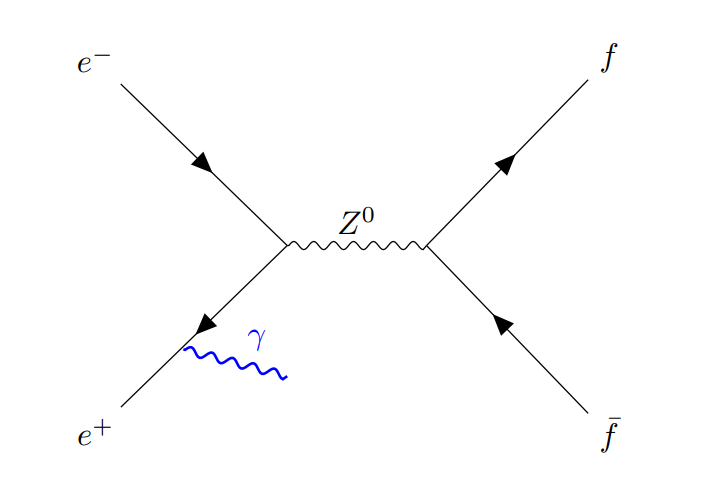
\includegraphics[width=\textwidth]{background1}
    \caption{Initial state radiation (ISR)}
\end{subfigure}
%\hfill
\begin{subfigure}{0.45\textwidth}
    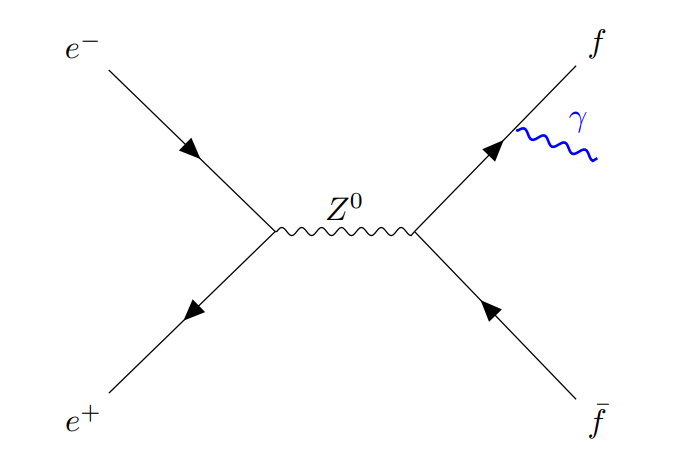
\includegraphics[width=\textwidth]{background2}
    \caption{Final state radiation (FSR)}
\end{subfigure}
%\hfill
\begin{subfigure}{0.45\textwidth}
    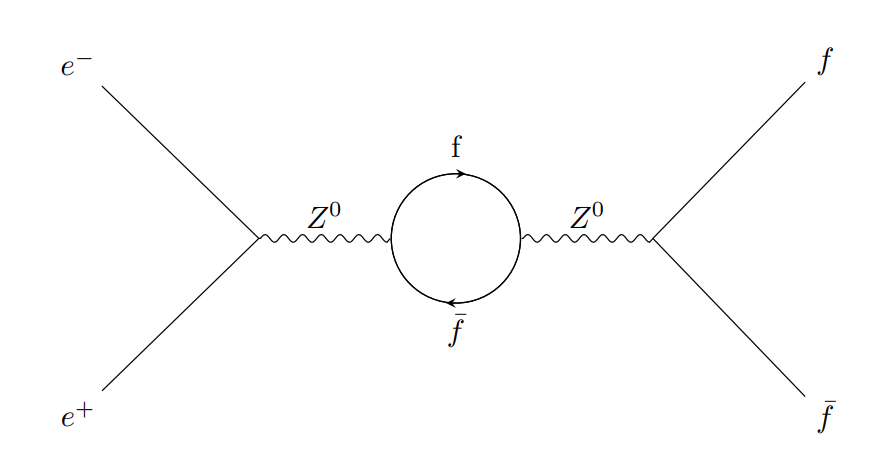
\includegraphics[width=\textwidth]{background3}
    \caption{$Z^{0}$ propagator correction}
\end{subfigure}
%\hfill
\begin{subfigure}{0.45\textwidth}
    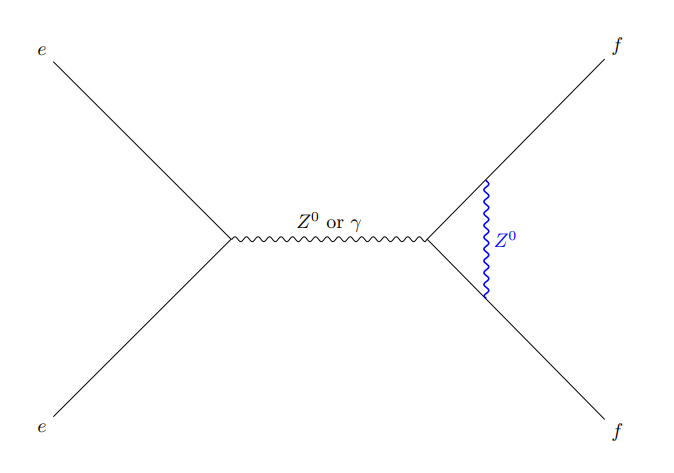
\includegraphics[width=\textwidth]{background4}
    \caption{$Z^{0}$ vertex correction}
\end{subfigure}       
\caption{Some examples of radiative corrections \cite{UB}}
\label{fig:backfig}
\end{figure}

\subsection{Important Parameters of a Resonance Particle}

\section{High Energy Colliders}
The Large Electron Positron Collider (LEP) was built at CERN, with one of its major goals being making high precision measurements of the parameters of the $Z^{0}$ boson, such as its mass, decay width and angular distributions of final state particles produced from $Z^{0}$ decays. As such, for most of its period of operation from 1989 to 1995, it produced $e^{+}e^{-}$ collisions at centre of mass energies very close to the $Z^{0}$ resonance and about 17 million $e^{+}e^{-}\rightarrow Z^{0}$ events were recorded in this time frame \cite{thomson_2013}. It was built in such a manner that the electron-positron collisions took place at four different points in the circular collider, and hence four such detectors were used in this experiment: ALEPH (Apparatus for LEP PHysics), DELPHI (DEtector with Lepton, Photon and Hadron Identification), L3 (Third LEP experiment) and OPAL (Omni-Purpose Apparatus for LEP). 

The components of the OPAL detector shall be described in further detail in this Section, since this experiment focuses on analysis of data collected by the OPAL.

\subsection{The OPAL Detector}
\begin{figure}[H]
\centering
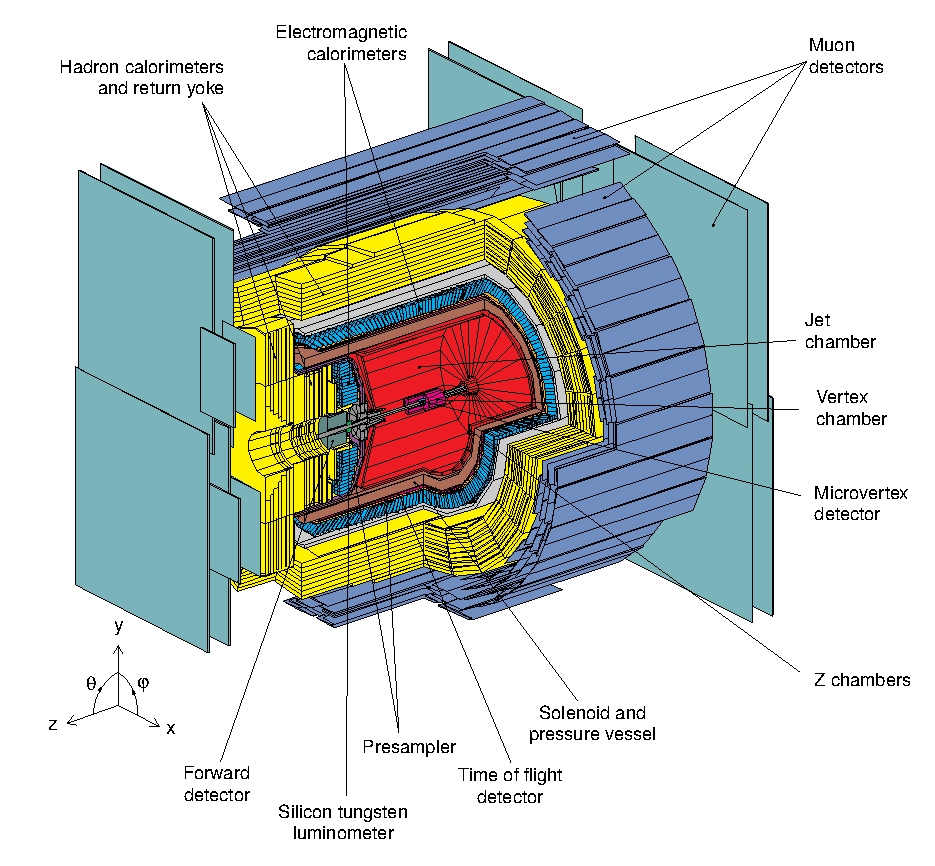
\includegraphics[width=0.7\textwidth]{OPAL1}
\caption{The OPAL Detector and its various components}
\label{fig:OPAL}
\end{figure}

For analysis of events arising from this detector, a right handed coordinate system is followed. The origin is fixed at the point where $e^{+}e^{-}$ collisions take place, the $x$ axis points horizontally in the direction of the center of the LEP, while the z axis is defined to lie along along the beam path and the y axis is then just perpendicular to the $x-y$ plane as usual. $\theta$, the polar angle is the angle between the $y$ and $z$ axes and the azimuthal angle $\phi$ is the counterclockwise angle between the $x$ and $y$ directions. The OPAL detector and this coordinate system is displayed in Figure \ref{fig:OPAL}.

Starting from the origin, as the $e^{+}e^{-}$ collision products fly outwards, various detector components are encountered which serve to detect the type and various characteristics of the final state particles. These primary detector components are discussed here in brief:
\begin{itemize}
\item \textbf{Vertex detector:}
\item \textbf{Jet chamber:}
\item \textbf{z chambers:}
\item \textbf{Time of flight (TOF) system:}
\item \textbf{Electromagnetic calorimeter (ECAL):}
\item \textbf{Hadron calorimeter (HCAL):}
\item \textbf{Muon detector:}
\end{itemize}
